\documentclass[11pt,a4paper,twoside]{report}
\usepackage[margin=1in, headheight=14pt]{geometry}
\usepackage{amsfonts,amsmath,amssymb,suetterl}
\usepackage{physics}
\usepackage{lmodern}
\usepackage[T1]{fontenc}
\usepackage{fancyhdr}
\usepackage{float}
\usepackage[utf8]{inputenc}
\usepackage{fontawesome}
\usepackage{enumerate}
\usepackage{graphicx}

\usepackage{pgfplots}
\usepackage{tikz}
\pgfplotsset{compat = newest}
\usetikzlibrary{decorations.text, positioning, arrows.meta}
\usepgfplotslibrary{fillbetween}

\DeclareUnicodeCharacter{2212}{-}

\usepackage{mathrsfs}
\usepackage[nodisplayskipstretch]{setspace}

\setstretch{1.5}
\renewcommand{\footrulewidth}{0pt}

\parindent 0ex
\setlength{\parskip}{1em}

\fancyfoot{}
\setcounter{chapter}{2}
\setcounter{section}{-1}

\pagestyle{fancy}

% title page
\long\def\mytitle{
	\begin{titlepage}
		\begin{center}
			\Huge Queen Mary\\
			\LARGE University of London
		\end{center}

		\vspace*{\stretch{1}}

		\begin{singlespace}
			{\centering
					{\huge\bfseries MTH5123 Differential Equations\\}
					\vspace{0.5cm}

					{\Large Lecture Notes\\}
					\vspace{0.5cm}

					{\Large Week 3}

					\vfill
					\LARGE Weini Huang
					\vspace{0.5cm}
					
					\LARGE School of Mathematical Sciences\\
					\LARGE Queen Mary University of London\\

					\vspace{0.5cm}
					\LARGE Autumn 2020\\
					}
		\end{singlespace}
	\end{titlepage}
}

\begin{document}
	\pagestyle{empty}
	\mytitle

	\pagestyle{fancy}
	\fancyhead[LE,RO]{\thepage}
	\fancyhead[LO]{\nouppercase \rightmark}

	%
  \chapter*{2 Initial value problem for first-order ODEs: existence and uniqueness of solutions}
	%
	In the previous chapter we have studied a few types of ODEs whose solutions $y(x)$ or $y(t)$ we were able either to write down explicitly, or to characterize implicitly in terms of a given function of two variables, e.g. as $F(x, y) = C$. The class of ODEs for which this can be done is however rather small. Most ODEs which are encountered in practice can not be solved in this or similar ways. If, however, we have an ODE for which we know that a solution exists, we may proceed to investigate its properties (e.g., the behaviour of $y(t)$ for large $t \to \infty$) \textit{regardless of whether we know the explicit form for the solution}. The corresponding methods are known as a \textit{qualitative study} of ODEs, and some of them will be briefly discussed later on in this module.\\
	Another important aspect is the \textbf{uniqueness} of a solution. For this we first need to define the \textit{initial value problem} for a first-order ODE. Such a problem asks to find a function $y(x)$ solving a given ODE by taking a specific value $y = b$ at the argument $x = a$. That is, the solution must satisfy the \textit{initial value} $y(a) = b$. We have seen for first-order ODEs like $\frac{dy}{dx} = f(y, x)$ that the general solution always has a \textbf{single} free parameter, which is the constant of integration. Solving an initial value problem requires to determine this free parameter by using the given initial condition $y(a) = b$.

  \section{Initial Value Problem}
	\textbf{Example:}\\
	Consider the first order separable ODE
	$$
	\frac{dy}{dx} = \frac{1}{2y}.
	$$
	Its solution is found to be $y(x)=\pm \sqrt{x+C}$ with arbitrary $C$. For this example, the initial condition $y(a) = b$ yields $b=\pm \sqrt{a+C}$ which is satisfied if $C=b^2-a$. Hence the solution to the initial value problem is given by
	$$
	y(x)
	=
	\begin{cases}
		\qquad \sqrt{x+b^2-a}, &\text{if}\ b>0\\
		\qquad -\sqrt{x+b^2-a}, &\text{if}\ b<0\\
		\text{both}\ \sqrt{x-a}\ \text{and}\ -\sqrt{x-a}, &\text{if}\ b=0\\
	\end{cases}
	$$
	We see that for $b = 0$ there are \textbf{two} solutions of the initial value problem, whereas for all other values of $b \ne 0$ there is \textbf{only one} solution. In the latter case we say that the solution is \textbf{unique}.\\
	By a \textbf{unique solution} we mean the following:\par
	\textbf{Definition:}\\
	An initial value problem for an ODE with initial condition $y(a) = b$ has a \textbf{unique} solution if for any two solutions $y_1(x)$ and $y_2(x)$ satisfying the same initial condition $y_1(a) = y_2(a) = b$, there exists a positive number $A > 0$ such that
	$$
	y_1(x) = y_2(x), \quad \forall x \in (a − A, a + A).
	$$
	In other words, uniqueness implies that two such solutions are \textbf{identical} for all $x$ in the hole interval $|x − a| < A$ for some $A > 0$.\par
	We have already seen that for some initial conditions solutions to initial value problems may not be unique.\par
	\textbf{Example:}\\
	Consider the first order ODE
	$$
	\frac{dy}{dx} = 3y^{2/3}
	$$
	with initial condition $y(0) = 0$. Obviously, $y(x) = 0$ is a solution to this initial value problem. On the other hand, this is a separable ODE, which in fact we have solved before: By separating the variables we found $y^{1/3} = x + C$, hence we have a family $\mathcal{F}$ of solutions $y = (x+C)^3$. Obviously, $y=x^3$ belongs to this family and also satisfies the above initial condition. Consequently, the solution to our initial value problem $y(0) = 0$ is \textit{not unique}. Similarly, for the initial value problem $y(a) = 0$ there are two solutions passing through the point $(a, 0): y(x) = 0$ and $y(x) = (x-a)^3$; see Fig. 2.1. Moreover, the curve $M_1N_1 \cup N_1N_2 \cup N_2K_2$, which is a mix between both these basic solutions, is another solution, as the left and the right derivatives at $N_1$ and $N_2$ are equal.

	%
	\begin{figure}[H]
		\centering
		\begin{tikzpicture}
			\begin{axis}[
				scale = 1.2,
				xmin = -5, xmax = 5,
				ymin = -7.5, ymax = 7.5,
				axis lines* = center,
				xtick = {0}, ytick = \empty,
				clip = false,
				]
				% Indifference curves
				\addplot[domain = -4.15:4.15, restrict y to domain =-7.3:7.3, samples = 400]{(x+2)^3};
				\addplot[domain = -2.25:2.25, restrict y to domain =-7.3:7.3, samples = 400]{x^3};
				\addplot[domain = -0.15:4.15, restrict y to domain =-7.3:7.3, samples = 400]{(x-2)^3};
				\addplot[domain = 1.8:6.1, restrict y to domain =-7.3:7.3, samples = 400]{(x-4)^3};
				% Labels
				\node [right] at (current axis.right of origin) {$x$};
				\node [above] at (current axis.above origin) {$y$};
				\node at (0.15,-0.4) {$0$};
				\node at (1.8,-0.5) {$a$};
				\node at (2,0.5) {$N_1$};
				\node at (4,0.5) {$N_2$};
				\node at (2.4,7.6) {$x^3$};
				\node at (4.4,7.6) {$K_1$};
				\node at (6.4,7.6) {$K_2$};
			\end{axis}
		\end{tikzpicture}
		\caption{Sketch of the solutions $y=(x+C)^3$ to the ODE $y^\prime = 3y^{2/3}$.}
	\end{figure}
	%
	\subsection{Picard-Lindel\"{o}f Existence and Uniqueness Theorem for I.V.P}
	Uniqueness of solutions is important for a number of reasons. Suppose we are able to find by some technique a one-parameter family $\mathcal{F}$ of solutions $y = y\mathcal{F}(x)$ of a first-order ODE. Furthermore, suppose for any point $(a, b)$ in some domain $\mathcal{D}$ of the $xy$ plane we can always find a solution in our family $\mathcal{F}$ which satisfies $y\mathcal{F}(a) = b$. If we know that uniqueness holds, then our family $\mathcal{F}$ of solutions must contain \textbf{all} desired solutions to our ODE, and we need look no further for other solutions.\\
	Uniqueness will also be of importance if, for instance, we wanted to approximate a solution numerically. If two \textit{different} solutions passed through a point, then successive approximations could very well jump from one solution to the other - with misleading consequences. It is therefore important to know under which conditions one can expect an ODE to have a unique solution for a specified initial condition. In case of first-order ODEs the answer is largely given by the \textbf{Picard-Lindel\"{o}f Existence and Uniqueness Theorem}, which we state without proof:\par
	\textbf{Theorem:} Picard-Lindel\"{o}f Existence and Uniqueness Theorem\\
	Consider the initial value problem
	%
	\begin{equation}
		\frac{dy}{dx} = f(x,y) \quad \text{with} \quad y(a) = b
	\end{equation}
	%
	Consider the IVP (2.1) on a rectangular domain $\mathcal{D}$ of the form $|x − a| \leq A$ and $|y − b| \leq B$(see Fig. 2.2), then it has \textbf{one and only one} solution in $\mathcal{D}$ provided the following two conditions are satisfied:
	%
	\begin{itemize}
		\item The function $f(x, y)$ is \textit{continuous} in $\mathcal{D}$ and therefore bounded: $|f(x, y)| \leq M\ \forall (x, y) \in \mathcal{D}$ for some positive constant $M > 0$. We also have to impose the restriction $A \leq B/M$ on the width of $\mathcal{D}$.
		\item  It has \textit{bounded derivative} $\frac{\partial f}{\partial y}$ everywhere in $\mathcal{D}$, that is, the value $K=\max _{(x,y)\in \mathcal{D}}\left\lvert \frac{\partial f}{\partial y}\right\rvert $ is finite: $0<K<\infty$.
	\end{itemize}
	\textbf{Note:}\\
	To see where the condition $A \leq B/M$ comes from one needs to go through the proof. If the derivative $\frac{\partial f}{\partial y}$ is \textit{continuous} everywhere in $mathcal{D}$ then it is necessarily bounded.\\
	The second condition is known as the \textit{Lipschitz condition} and the constant $K$ as the \textit{Lipschitz constant}.
	%
	\begin{figure}[H]
		\centering
		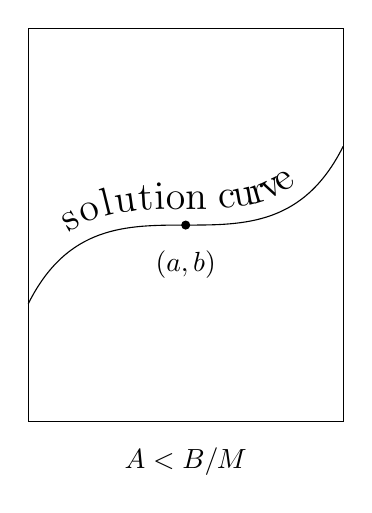
\begin{tikzpicture}
			\draw (0,0) rectangle (4,5);
			\draw (0,1.5) .. controls (1,3.5) and (3,1.5) .. (4,3.5);
			\draw[decoration={
				text along path,
				text={|\Large| solution curve},
				text align={center},
				raise=0.2cm},decorate] (0,1.5) .. controls (1,3.5) and (3,1.5) .. (4,3.5);
			\draw[fill] (2,2.5) circle [radius =0.05];
			\node at (2,2) {$(a,b)$};
			\node at (2,-0.5) {$A<B/M$};
		\end{tikzpicture}
		%
		\caption{Sketch of a a rectangular space $\mathcal{D}:{a − A \leq x \leq a + A, b − B \leq y \leq b + B}$, where uniqueness is ensured due to the Picard-Lindel\"{o}f theorem.}
	\end{figure}
	%
	\textbf{Example:}\\
	For the example of non-uniqueness given above, with $f(y)=3y^{2/3}$ we have $\frac{\partial f}{\partial y} = 2y^{-1/3}$ which \textit{diverges} close to $y=b=0$ thus violating the Lipschitz condition and hence invalidating the Picard-Lindel\"{o}f theorem.\par
	\textbf{Note:}\\
	It is important to understand that the existence and uniqueness properties of the solution are guaranteed by the Picard–Lindel\"{o}f theorem only \textit{locally}, i.e. sufficiently close to the point $(a, b)$. In no way it implies existence and uniqueness everywhere.\par
	\textbf{Example:}\\
	Consider the initial value problem
	$$
	\frac{dy}{dx} = f(x,y), \quad y(0) = 1,
	$$
	where $f(x, y)$ is defined as
	$$
	f(x,y) = x^2|y|^{\frac{1}{3}},
	$$
	%
	\begin{enumerate}[\bfseries i)]
		\item Explain why the Picard-Lindel\"{o}f Theorem guarantees the existence and uniqueness of the solution to the above I.V.P on a rectangular domain $\mathcal{D} = (|x| \leq A, |y − 1| \leq B)$ in the $xy$ plane only for heights $B$ satisfying $0 < B < 1$. Find the value of the Lipschitz constant $K$ for the above problem for given $A$ and $B$.
		\item Suppose that the height $B$ of $\mathcal{D}$ is given and satisfies $0 < B < 1$. Show that the width A must then satisfy the inequality
		$$
		0 < A \leq \frac{b^{1/3}}{(1+B)^{1/9}}
		$$
	\end{enumerate}
	%
	\textbf{Solution:}
	\begin{enumerate}[\bfseries i)]
		\item The right-hand side of $f(x, y)$ depends on $|y|$, hence formally it is defined separately for positive and negative values of $y$:
		$$
		f(x,y)
		=
		\begin{cases}
			x^2y^{1/3}, &y>0\\
			x^2(-y)^{1/3}, &y<0
		\end{cases}
		$$
		This polynomial expression is continuous everywhere in $\mathcal{D}$, as nothing goes wrong at $y = 0$:
		$$
		\lim_{y \to 0^+}f(x, y) = \lim_{y \to 0^-}f(x,y)=0.
		$$
		On the other hand, the derivative
		$$
		\frac{\partial f}{\partial y}
		=
		\begin{cases}
			\frac{1}{3}x^2y^{-2/3} & \text{for} \quad y>0\\
			-\frac{1}{3}x^2(-y)^{-2/3}, & \text{for} \quad y<0
		\end{cases}
		$$
		is defined and finite everywhere \textit{except} at $y = 0$ where it diverges. Therefore this point has to be \textit{excluded} from $\mathcal{D}$ to ensure the conditions of the Picard-Lindel\"{o}f Theorem. This means the interval $|y − 1| \leq B$ (or, equivalently, $y \in [1 − B, 1 + B]$ with $B > 0$) cannot contain $y = 0$, which is only possible for $0 < B < 1$.\\
		The Lipschitz constant K can be found according to
		\begin{equation*}
			\begin{split}
				K &= \max_{(x,y)\in\mathcal{D}}\left\lvert \frac{\partial f}{\partial y}\right\rvert \\
		&= \max \left[x^2\right]_{-A \leq x \leq A} \cdot \max\left[\frac{1}{3}|y|^{-2/3}\right]_{1-B\leq y \leq 1+B}\\
		&= \frac{A^2}{3(1-B)^{2/3}}
			\end{split}
		\end{equation*}
		\item The modulus of the function $|f(x,y)| = x^2|y|^{1/3}$ on the right-hand side of the ODE grows with both $|x|$ and $|y|$, hence for a given $B$ its maximum $M$ in $\mathcal{D}$ is achieved for $x = \pm A$ and $y = 1 + B$:
		$$
		M = \max_{(x,y)\in \mathcal{D}}|f(x,y| = A^2(1+B)^{1/3}
		$$
		This in turn implies that the width $A > 0$ should satisfy $A \leq B/M = \frac{B}{A^2(1+B)^{1/3}}$. Rearranging gives
		$$
		A^3\leq \frac{B}{(1+B)^{1/3}}\quad \text{or} \quad 0<A<\frac{b^{1/3}}{(1+B)^{1/9}}.
		$$
	\end{enumerate}
	%
	\section{Systems of first-order ODEs}
	Our main goal in this section is to extend the previous theory of existence and uniqueness to systems of $n$ first-order ODEs for $n$ unknown functions $y_1(t), y_2(t),\ldots ,y_n(t)$ written in the \textbf{normal form}
	%
	\begin{equation}
		\begin{cases}
			\dot{y}_1 = f_1(t, y_1, \ldots, y_n)\\
			\dot{y}_2 = f_2(t, y_1, \ldots, y_n)\\
			\qquad \quad \ldots\\
			\qquad \quad \ldots\\
			\dot{y}_n = f_n(t, y_1, \ldots, y_n)
		\end{cases}
	\end{equation}
	%
	For sake of brevity we consider only the case $n = 2$. Using vector notation we can write down any such system in normal form as
	%
	\begin{equation}
		\dot{\vb{y}} = \vb{f}(t,\vb{y}),\quad
		\vb{y} =
		\begin{pmatrix}
			y_1\\
			y_2
		\end{pmatrix}, \quad
		\vb{f} = 
		\begin{pmatrix}
			f_1(t,y_1,y_2)\\
			f_2(t,y_1,y_2)
		\end{pmatrix}.
	\end{equation}
	%
	By imposing the \textbf{initial conditions} at $t = a$
	\begin{equation}
		y_1(a) = b_1, \quad
		y_2(a) = b_2,
	\end{equation}
	where $b_1$ and $b_2$ are given constants, we can formulate the initial value problem for the system (2.3).
	\subsection*{The equivalence of n first-order ODEs to 1 n-th order ODE}
	The system (2.2) is \textit{very fundamental}, as \textit{any} $n$-th order ODE of the form
	%
	\begin{equation}
		\frac{d^ny}{dx^n} = F\left(x,y,\frac{dy}{dx},\frac{d^y}{dx^2},\ldots, \frac{d^{n-1}y}{dx^{n-1}}\right)
	\end{equation}
	%
	is in fact equivalent to a system of the form (2.2). To see this, introduce the notation $t \equiv x$ and further denote
	%
	\begin{equation}
		y_1(t) \equiv y(x),\ 
		y_2(t) \equiv \frac{dy}{dx},\ 
		y_3(t) \equiv \frac{d^2y}{dx^2},\ldots,
		y_n(t)\equiv \frac{d^{n-1}y}{dx^{n-1}}.
	\end{equation}
	%
	The functions $y_1(t),\ldots ,y_n(t)$ then satisfy the $(n − 1)$ relations
	%
	\begin{equation}
		\dot{y_1}(t) = y_2(t),\ 
		\dot{y_2}(t) = y_3(t),\ \ldots,\ 
		\dot{y_{n-1}}(t) = y_n(t)
	\end{equation}
	%
	such that (2.5) takes the form, in the new notation,
	%
	\begin{equation}
		\dot{y_n}(t) = F(t, y_1, y_2, y_3, \ldots,y_n).
	\end{equation}
	%
	Equations (2.7)-(2.8) are exactly of the form of (2.2) with
	%
	\begin{equation}
		\begin{gathered}
			f_1(t,\vb{y})=y_2, \quad f_2(t,\vb{y})=y_3,\quad \ldots\\
			\ldots, \quad f_{n-1}(t,\vb{y})=y_n, \quad f_n(t,\vb{y})=F(t,y_1,y_2,y_3,\ldots,y_n).
		\end{gathered}
	\end{equation}
	%
	\textbf{Example:}\\
	Transform the second order ODE
	$$
	\frac{d^2y}{dx^2} = 6y-4\frac{dy}{dx}
	$$
	to a system of first-order ODEs.\par
	\textbf{Solution:}\\
	By using $t \equiv x$, identify according to (2.6)
	$$
	y_1(t)\equiv y(x),\quad y_2(t)\equiv \frac{dy}{dx}.
	$$
	Differentiate these equations, cf. (2.7):
	$$
	\dot{y_1}(t) = y^\prime = y_2(t),\ \dot{y_2}(t)=y^{\prime\prime}.
	$$
	According to (2.8) we then obtain the system of two first-order ODEs
	$$
	\dot{y_1}(t) = y_2(t),\ \dot{y_2}(t) = 6y-4y^\prime = 6y_1-4y_2.
	$$
	This example belongs to an important special class of $n$-th order ODEs, linear ODEs of second order (here with constant coefficients), which we will discuss in more detail in the next chapter.
\end{document}